\begin{center}
  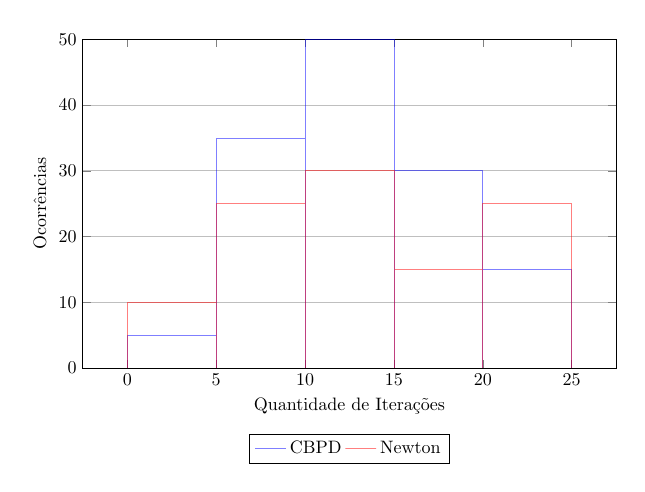
\begin{tikzpicture}[scale = 0.65]
  \begin{axis}[
    width=12cm,
    height=8cm,
    xlabel={Quantidade de Iterações},
    ylabel={Ocorrências},
    ymajorgrids=true,
    ymin=0,
    ymax=50,
    legend style={at={(0.5,-0.2)}, anchor=north, legend columns=-1},
  ]

    \addplot+[blue, opacity=0.5, ybar interval, mark=no] plot coordinates { 
      (0, 5)
      (5, 35)
      (10, 50)
      (15, 30)
      (20, 15)
      (25, 0)
    };
    
    \addplot+[red, opacity=0.5, ybar interval, mark=no] plot coordinates { 
      (0, 10) 
      (5, 25) 
      (10, 30) 
      (15, 15) 
      (20, 25) 
      (25, 0) 
    };

    \legend{CBPD, Newton}

  \end{axis}
\end{tikzpicture}  
\end{center}
